\section{Mini-Project B}
This project is for CS students only. Of course, if you'd like to attempt, you can.\\

\subsection{Scenario}
The biology student appreciates the work you have done developing a rough prototype. Their research has started gaining ground, and more people are becoming interested in their research. Because you did such a good job of developing the base system, the biology student has asked you to develop a means of a system where anyone can access their data. Being competent developers, well aware of web development, as well as being aware of the world of embedded systems you decide to use MQTT to transfer data. You want to make the system as accessible as possible, so you decide to use a low-cost Raspberry Pi to host a Node-Red server. For the sake of the prototype, you create a hotspot on the Raspberry Pi that people can connect to in order to access the server. You decide on the following design, as shown in Figure \ref{fig:NodeRed}:

\begin{figure}[H]
\centering
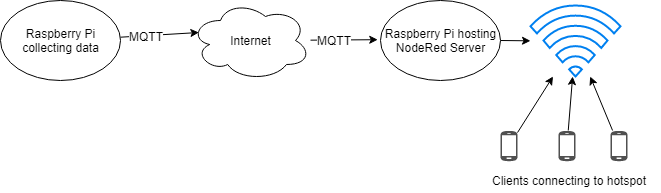
\includegraphics[width=0.8\columnwidth]{Figures/NodeRed}
\caption{Project B System Overview}
\label{fig:NodeRed}
\end{figure}

\subsubsection{Overview}
For this task, two Raspberry Pi's are required.One is to act as an MQTT broker, publishing the data gathered as per Mini Project A. The second is to act as an MQTT client that is subscribed to the first Pi and can be used to configure thresholds and display data using Node Red. A webpage must be hosted on the second Pi, and it's WiFi interface should be turned into an access point. Devices should be able to connect to this access point, and view the web page.

Essentially, this is a repeat of the first project, but using a second Raspberry Pi with MQTT and Node Red as opposed to Blynk.

\subsubsection{Outcomes}
You will learn about:
\begin{itemize}
    \item MQTT
    \item NodeRed
\end{itemize}

\subsubsection{Deliverables}
At the end of this practical, you must
\begin{itemize}
    \item Demonstrate your implementation to a tutor. They will log in to your hotspot through their phone, view values, and adjust thresholds.
    \item Submit a short write up. See the marking guide in section \ref{sec:ProjBMarks}
\end{itemize}

\subsubsection{Hardware Required}
You require the hardware from Project A, as well as a secondary Pi.

\subsubsection{Software Requirements}
\begin{itemize}
    \item You need to use an MQTT broker to publish and subscribe to messages relating to your practical. 
    \item You need to create a Node Red server that displays your data gathered from the first Raspberry Pi. 
    \item You will also need to have an option to adjust the alarm threshold from the NodeRed server.
\end{itemize}

\subsubsection{Marking Guide}
\label{sec:ProjBMarks}
TBD

\subsubsection{Project B Validation Guide}
\label{sec:ProjBValidation}
TBD
